\subsection{Simulation settings}

\begin{figure}[h!]\label{fig:scenarios}
    \centering
    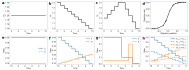
\includegraphics[width=1\textwidth]{figures/scenarios.pdf}
    \caption{The different scenarios considered in the simulation studies. (a) Epi-1 — constant reproduction number; (b) Epi-2 — linearly decreasing reproduction number; (c) Epi-3 — non-monotonic reproduction number; (d) Epi-4 — migration rates between five populations predicted by a continuous covariate; (e) FBD-1 — constant speciation and extinction rates; (f) FBD-2 — linearly decreasing speciation rate and linearly increasing extinction rate; (g) FBD-3 — non-linear speciation rate with a spike in the extinction rate; (h) FBD-4 — linearly decreasing speciation rate and linearly increasing extinction rate across four groups of species defined by two binary traits (only one trait affects diversification).}
\end{figure}

We benchmarked our approach on \textbf{eight simulation scenarios}, grouped into two classes of multi-type birth-death models~\cite{stadler2013uncovering}: epidemiological processes (with removal after sampling) and fossilized birth-death (FBD) processes~\cite{Heath2014FBD} (with ancestor sampling and complete present-day sampling). Figure~1 graphically illustrates the inference targets for each scenario with respect to their predictors.

All epidemiological scenarios (a-d) share: the same become-uninfectious rate \( \delta = \mu + \psi = 0.07 \), the same sampling proportion \( s = \frac{\psi}{\mu + \psi} = 0.15 \), and the same simulation time \( T = 250 \). Scenarios \emph{a-c} are characterized by a unique population, and the inference task is to estimate a piece-wise constant (skyline) reproduction number \( R_t = \frac{\lambda}{\mu + \psi} \) using time as predictor. \( R_t \) is constant in scenario \emph{a}, linearly decreasing in scenario \emph{b}, and non-monotonic in scenario \emph{c}. Scenario \emph{d} is characterized by five populations, with constant reproduction numbers for each of them (respectively, 0.8, 1.0, 1.2, 1.4 and 1.6), and the task is to infer the 20 pairwise migration rates using a continuous covariate as migration predictor. To generate these rates, the migration predictors were first sampled from a uniform distribution \( \mathcal{U}(-1, 1) \) and then mapped into target migration rates using a sigmoid function.

All FBD scenarios (e-h) assume the same constant ancestor sampling rate \( \psi = 0.2 \) and simulation time \( T = 35 \), and the inference task is to estimate skyline speciation and extinction rates across 10 time bins. Predictors are given by time and, for scenario \emph{h}, by two additional binary traits. Scenario \emph{e} assumes constant speciation and extinction rates; scenario \emph{f} features a linearly decreasing speciation rate and a linearly increasing extinction rate; scenario \emph{g} models nonlinear decreases in the speciation rate, while the extinction rate exhibits a sharp upward spike in the second half of the simulation. Scenario \emph{h} involves four different groups of species, distinguished by the combination of values of two binary traits. However, the second of these traits does not affect evolutionary dynamics, meaning that the four populations can be further grouped into two pairs that share identical speciation and extinction rates. For each pair, the speciation rate decreases linearly while the extinction rate increases linearly.

To assess the robustness of our approach to misspecifications in the predictor set—particularly with respect to the inclusion of irrelevant predictors—we incorporated an additional randomly generated predictor into all simulation studies. This predictor was constructed randomly and independently of the inference target, and resampled for each tree. In scenario \emph{d}, it consisted of a uniformly distributed random value in \( [1, -1] \) for each of the 20 population pairs, whereas for all other (skyline) scenarios, it was defined as a random walk with standard normal increments across the time bins.
